%++++++++++++++++++++++++++++++++++++++++
% Don't modify this section unless you know what you're doing!
\documentclass[letterpaper,12pt]{article}
\setlength{\parindent}{4ex}
\setlength{\parskip}{1ex}

\usepackage{graphicx}
\usepackage{indentfirst}
\usepackage{tabularx} % extra features for tabular environment
\usepackage{subfigure} 

\usepackage{caption} % Spacing between caption (title) and actual table
\captionsetup[table]{skip=10pt}

\usepackage{amsmath}  % improve math presentation
\usepackage{graphicx} % takes care of graphic including machinery
\usepackage{pgfplots}
\usepackage[margin=1in,letterpaper]{geometry} % decreases margins
\usepackage{cite} % takes care of citations
\usepackage[final]{hyperref} % adds hyper links inside the generated pdf file
\hypersetup {
	colorlinks=true,       % false: boxed links; true: colored links
	linkcolor=blue,        % color of internal links
	citecolor=blue,        % color of links to bibliography
	filecolor=magenta,     % color of file links
	urlcolor=blue         
      }
      \setcounter{tocdepth}{3}

\usepackage{pgfplots}      


% ++++++++++++++++++++++++++++++++++++++++

\begin{document}

\title{CS 7641 Machine Learning \\
		\ Assignment 1 }
\author{David Yun}
\date{September 23, 2018}
\maketitle

\begin{abstract}
  The implementation (in Python2.6 or Python3, depending on the algorithm), and basic fundamentals behind the following Machine Learning Algorithms will be discussed in detail:  
  \begin{enumerate}
    \item Decision trees with some form of pruning
    \item Neural Networks
    \item Boosting
    \item Support Vector Machines (SVM)
    \item k-Nearest Neighbors (kNN)
      
    \end{enumerate}

    The full code files are available on github\footnote{David Yun's Github: \url{https://github.com/tree-fiddy/Assignment_1}}
    Please refer to the README.txt file for concise instructions on how to run the python files associated with each of the aforementioned algorithms.  Further details behind the datasets, including where to download them, are provided in the README.  

\end{abstract}

\tableofcontents

\section{Datasets}
The two datasets used are both sourced from the UCI Machine Learning Repository.  The first one, the \href{http://archive.ics.uci.edu/ml/datasets/credit+approval}{Credit Approval Data Set} is a smaller dataset with 690 instances, and 15 attributes.  As a full time employee at American Express, credit approval is highly relevant to my job.  As such, I wanted to take this opportunity to see how Machine Learning can be directly applied to credit approval data.  The second dataset, the \href{https://archive.ics.uci.edu/ml/datasets/MoCap+Hand+Postures#}{MoCap Hand Postures Data Set} is a much larger dataset with 78,095 instances, and 38 features.  This dataset classifies 5 different hand gestures using markers attached to fingers of a glove in a motion capture environment.  The application of Machine Learning here is interesting because it provides a rudimentary step in the direction towards Virtual Reality- a burgeoning field directly applying Machine Learning to read \& track objects.

I thought it would behoove me to use two very different datasets, both in scope, and size, to truly gain an understanding of the usefulness of Machine Learning.  Not all models are built the same, and not all datasets benefit from a given model.  Thus, getting the opportunity to apply the same, or similar, models on two fundamentally different datasets would help uncover where certain models prove useful, and where the same models might prove inadequate.  

\section{Decision Trees}

The implementation of Decision Trees was borrowed from my previous coursework in CSE6242 (Data Visualization) with minor tweaks.
\textbf{Cross-Validation} is done without the need for a training-validation split here because of the use of Random Forests, which is a collection of decision trees.  Random forests allow us to create a robust model with less variance which results in a reduction in overfitting\footnote{By averaging several decision trees, the result is a less likely chance of overfitting}.  With proper pruning (Entropy thresholds \& Max Depth), one can further reduce the variance of the model and further decrease the chance of overfitting.  The \textbf{dataset} used is the UCI Credit Approval Dataset\footnote{UCI Credit Approval Data Set: \url{http://archive.ics.uci.edu/ml/datasets/credit+approval}}.  Some small adjustments were made to the dataset, such as removing rows where data was missing.  

\subsection{Learning Curves Analysis}
The accuracy of our decision tree relies on our tolerance for pre-pruning.  In essence, one must specify \emph{when} to stop growing the tree.  On one extreme, we can set a condition to stop growing the tree once we reach a \emph{pure\footnote{A leaf is said to be ``pure'' if the leaf contains homogenous labels.  By extension, this equates to a situation where Entropy equals 0.}} leaf.  However, this will likely make the tree longer than need be.  A more depth-restrictive approach is to set an arbitrary threshold for Entropy in our Decision Tree, where we will halt further node and leaf generation if the current node produces leaves with Entropy values less than our specified threshold.  To ensure the efficacy of our pre-pruning process, we also incorporate a limit to the depth of our tree to 5.  This will handle extreme cases where our dataset is so large, that splitting across many features is possible. This also has the added benefit of dramatic performance improvement, without sacrificing accuracy, when compared to not setting a depth and letting the tree grow indefinitely.  The performance of our decision tree, while varying \text{threshold levels} is highlighted in Table \ref{table:PrePruningTable}.

\begin{table}[htb]
  \caption{Pre-Pruning Spec Performance (forest size = 50)}
  \label{table:PrePruningTable}
  \centering
  \begin{tabular}{|c|c|c|}
  
    \hline
    \hline
    \multicolumn{1}{c}{Entropy Threshold}
    &  \multicolumn{1}{c}{Model Accuracy} \\
    \cline{1-2}
    0.0 & 0.86 \\
    \cline{1-2}
    0.1 & 0.86 \\
    \cline{1-2}
    0.2 & 0.60 \\
    \cline{1-2}
    0.3 & 0.57 \\
    \cline{1-2}
    0.4 & 0.55 \\
    \cline{1-2}
    0.5 & 0.55 \\
    \cline{1-2}
    0.6 & 0.54 \\
    \cline{1-2}
    0.7 & 0.54 \\
    
    
    \cline{1-2}
  \end{tabular}
\end{table}

\begin{figure}
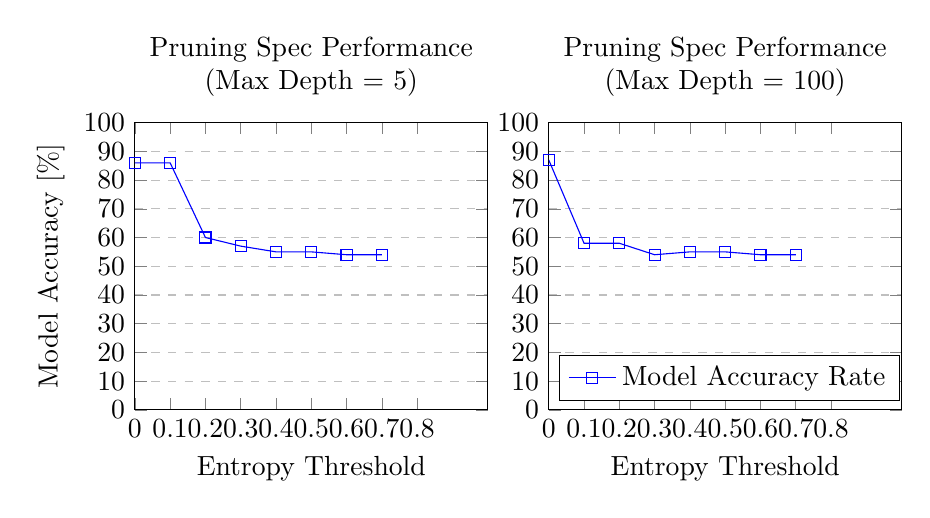
\begin{tikzpicture}[every axis/.append style={width=0.5\linewidth,title style={align=center}}]

  \begin{axis} [
    name = axis1,
    title = {Pruning Spec Performance \\ (Max Depth = 5)},
    xlabel = {Entropy Threshold},
    ylabel = {Model Accuracy [\%]},
    xmin = 0, xmax = 1,
    ymin = 0, ymax = 100,
    xtick={0,0.1,0.2,0.3,0.4,0.5,0.6,0.7,0.8},
    ytick={0,10,20,30,40,50,60,70,80,90,100},
    legend pos = south west,
    ymajorgrids=true,
    grid style = dashed
    ]
    \addplot[
    color = blue,
    mark = square,
    ]
    coordinates {
      (0.0,86)(0.1, 86)(0.2, 60)(0.3,57)(0.4,55)(0.5,55)(0.6,54)(0.7,54)
    };
  \end{axis}
  
  \begin{axis} [
    at={(axis1.outer north east)}, anchor=outer north west,
    name=axis2,
    title = {Pruning Spec Performance \\ (Max Depth = 100)},
    xlabel = {Entropy Threshold},
    %ylabel = {Model Accuracy [\%]},
    xmin = 0, xmax = 1,
    ymin = 0, ymax = 100,
    xtick={0,0.1,0.2,0.3,0.4,0.5,0.6,0.7,0.8},
    ytick={0,10,20,30,40,50,60,70,80,90,100},
    legend pos = south west,
    ymajorgrids=true,
    grid style = dashed
    ]
    \addplot[
    color = blue,
    mark = square,
    ]
    coordinates {
      (0.0,87)(0.1, 58)(0.2, 58)(0.3,54)(0.4,55)(0.5,55)(0.6,54)(0.7,54)
    };
    \legend{Model Accuracy Rate}
    
 
  \end{axis}
\end{tikzpicture}

\caption{Learning Curves} \label{fig:LearningCurves}
\end{figure}


As you can see, the model's accuracy reached an asymptote of around 50\% accuracy, which indicates that setting a higher threshold for Entropy renders this model's efficacy no better than a coin flip.  Thus, setting a pre-pruning specification is quite important here.  More notable is the fact that using the extreme case where Entropy must equal 0 before considering the tree complete yielded the same results as a 0.1 threshold.  However, computation times were slightly longer for this case, as more nodes had to be constructed until the threshold was met.  While in our dataset, it wasn't a huge factor, this is an important consideration one should make when building models on much larger data.  When the efficacy/accuracy of a model isn't compromised, any measures to speed up performance is a welcomed consideration.

You can also see that increasing the depth of the tree produced slightly better results \textbf{only} when we didn't set a threshold.  However, the computational time increased dramatically.  Moreover, setting entropy thresholds while allowing the tree to grow up to 100 levels deep caused this model to perform very poorly.

\subsection{Model Complexity Analysis}
Besides varying the Entropy Threshold \& Max Depth, we can also vary the \textbf{forest size} hyperparameter in our random forest.  Note here that we vary the hyperparameter, while holding the Entropy Threshold to 0.1 as supported by Figure \ref{fig:LearningCurves}.

\begin{figure}
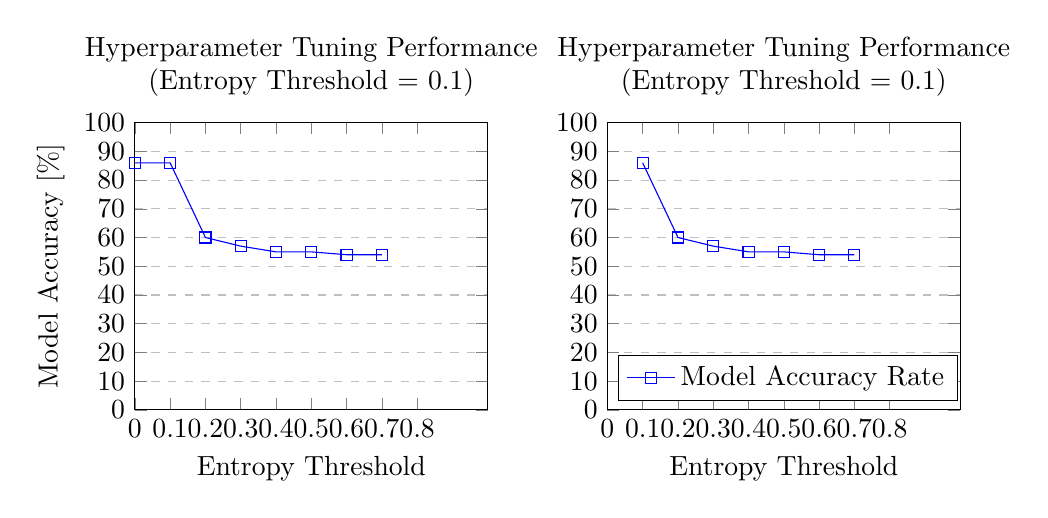
\begin{tikzpicture}[every axis/.append style={width=0.5\linewidth,title style={align=center}}]

  \begin{axis} [
    name = axis1,
    title = {Hyperparameter Tuning Performance \\ (Entropy Threshold = 0.1)},
    xlabel = {Entropy Threshold},
    ylabel = {Model Accuracy [\%]},
    xmin = 0, xmax = 1,
    ymin = 0, ymax = 100,
    xtick={0,0.1,0.2,0.3,0.4,0.5,0.6,0.7,0.8},
    ytick={0,10,20,30,40,50,60,70,80,90,100},
    legend pos = south west,
    ymajorgrids=true,
    grid style = dashed
    ]
    \addplot[
    color = blue,
    mark = square,
    ]
    coordinates {
      (0.0,86)(0.1, 86)(0.2, 60)(0.3,57)(0.4,55)(0.5,55)(0.6,54)(0.7,54)
    };
  \end{axis}
  
  \begin{axis} [
    at={(axis1.outer north east)}, anchor=outer north west,
    name=axis2,
    title = {Hyperparameter Tuning Performance \\ (Entropy Threshold = 0.1)},
    xlabel = {Entropy Threshold},
    %ylabel = {Model Accuracy [\%]},
    xmin = 0, xmax = 1,
    ymin = 0, ymax = 100,
    xtick={0,0.1,0.2,0.3,0.4,0.5,0.6,0.7,0.8},
    ytick={0,10,20,30,40,50,60,70,80,90,100},
    legend pos = south west,
    ymajorgrids=true,
    grid style = dashed
    ]
    \addplot[
    color = blue,
    mark = square,
    ]
    coordinates {
      (0.1,86)(0.1, 86)(0.2, 60)(0.3,57)(0.4,55)(0.5,55)(0.6,54)(0.7,54)
    };
    \legend{Model Accuracy Rate}
    
 
  \end{axis}
\end{tikzpicture}

\caption{Learning Curves} \label{fig:LearningCurves}
\end{figure}


\section{Artificial Neural Networks}

\subsection{Learning Curves Analysis}
We can further optimize our analysis by letting other parameters in our Neural Network to vary.  For one, we can tune our parameters through increasing both the depth and size of our hidden layers.  Looking at figure \ref{fig:ANN Complexity Curves}, you can see that our ANN model with 3 hidden layers, each of size 30 performs slightly better at lower iterations, but worse at higher number of iterations, as compared to specifying 1 hidden layer of size 1 node.  The overall conclusion here is that the simple model with 1 hidden layer using 1 node actually performs better than one with more hidden layers at high number of iterations.  

\begin{figure} %
  \centering
  \subfigure[3 Hidden Layers, 30 Nodes Each] {%
    \label{fig:ANN Complexity Curve Layer30x3}%
    \includegraphics[height=1.9in]{Neural_Nets/output/ANN_Accuracy_Rates3.png}}%
  \hspace{8pt}%
  \subfigure[1 Hidden Layer, 1 Node]{%
    \label{fig:ANN Complexity Curve}%
    \includegraphics[height=1.9in]{Neural_Nets/output/ANN_Accuracy_Rates4.png}}
  \caption{Complexity Curves:  Testing vs. Validation Sets w/ Varying Depth and Number of Hidden Layer Nodes}\label{fig:ANN Complexity Curves}
\end{figure}


The first figure in \ref{fig:ANN Complexity Curves} produces very promising results.  With 30 nodes in each of the 3 Hidden Layers, we can only achieve 80\% fit in the training set, and 80\% in the test set no matter the number of weight-adjustment iterations (backpropogation).  The performance is quite poor all around.  The right graph uses the $basicResults.best\_params\_$ method made available in scikitlearn to choose the best parameter for our ANN.  The best parameters are:  (1) L2 Penalty: 0.00316 (2) Hidden Layer Depth: 1 (3) Hidden Layer Size: 1 (4) Activation Function: RELU.  Note that the figure on the right suggests we can reach a generalizable and accurate (88\% test accuracy rate with 90\% training accuracy rate) model with anywhere between 1,024 to 2048 weight-adjustment iterations.  Figure \ref{fig:ANN Complexity Curve} also highlights the importance of back-propogation.  Giving our model time to make iterative adjustments to the weights drastically improves the model.   

\subsection{Model Complexity Analysis}
To get a basic understanding of how our model performed, we first start off with a ``basic'' neural net with the following specifications:  (1) 1 Hidden Layer of size 30.  (2) Activation Function = 'relu' (rectified linear unit function, returns f(x) = max(0,x)) (3) L2 Regularization Alpha = 0.  The figure in Figure \ref{fig:ANN Learning Curves} shows the results with the aforementioned specifications, but letting our L2 Regularization/Penalty term to vary between 0 \& 10.
Recall that the L2 Norm is essentially a squared error specification, and by it's nature, penalizes weights in a manner to reduce the likelihood of fitting the noise of the training data.  

\begin{figure} %
  \centering
  \subfigure[L2 Regularization = 0] {%
    \label{fig:ANN Learning Curve L2 = 0}%
    \includegraphics[height=1.9in]{Neural_Nets/output/ANN_Accuracy_Rates.png}}%
  \hspace{8pt}%
  \subfigure[L2 Regularization = 10]{%
    \label{fig:ANN Learning Curve L2 = 10}%
    \includegraphics[height=1.9in]{Neural_Nets/output/ANN_Accuracy_Rates2.png}}
  \caption{Learning Curves:  Training vs. Validation Sets w/ Varying Alpha (L2-Norm)}\label{fig:ANN Learning Curves}
\end{figure}

\section{k-Nearest Neighbors}
Classifying hand gestures based on relative position across 3-dimensional coordinate plane is a perfect candidate for kNN.  By measuring the coordinates of markers attached to each finger as a hand gesture (fist, point, grab ...etc.), one can reasonably identify general characteristics related to finger positioning associated with gestures across different users (or, hands).

\subsection{Learning Curves Analysis}
To get a sense of how effectively our kNN model learns across different sizes of our training set, we can compare the performance of our model as we increase the training set.  We will compare the outcomes of our model under 2 scenarios, where each scenario uses a different value for our hyper-parameter $k$.  We first start off with a ``basic'' implementation of kNN with the following specifications:  (1) Default k of 10.  (2) Distance = Manhattan (3) Weighting distance of training data uniformly. We then compare our results with the ``best'' implementation, as chosen by $GridSearchCV.best\_params\_$.  It turns out, $ k=1$, using the Manhattan distance weighted uniformly performs the best.  The figure in Figure \ref{fig:kNN Learning Curves} shows the results with the aforementioned specifications, but letting our $k$ vary from 10 to the optimum $k=1$ outputted via $GridSearchCV.best\_params\_$.  As you can see, setting $k=1$ generated perfect training sets (100\% training accuracy across all sample sizes).  In other words, our 1-NN perfectly classified our training data set.  This is largely expected, as 1-NN has low bias, and high variance, and generally produces results suggesting overfitting.  


\begin{figure} %
  \centering
  \subfigure[k = 10] {%
    \label{fig:kNN Learning Curve k = 10}%
    \includegraphics[height=2in]{KNN/output/kNN_Accuracy_Rates.png}}%
  \hspace{8pt}%
  \subfigure[k = 1]{%
    \label{fig:kNN Learning Curve k = 1}%
    \includegraphics[height=2in]{KNN/output/kNN_Accuracy_Rates2.png}}
  \caption{Learning Curves:  Training vs. Validation Accuracy w/ Varying Training Set Size}\label{fig:kNN Learning Curves}
\end{figure}

As you can see in figure \ref{fig:kNN Learning Curves}, our validation accuracy experiences a drastic improvement in accuracy as our training set size reaches ~6000.  Furthermore, we see overfitting occurring at both levels of $k=1$ and $k=10$, evidenced by the near perfect training scores.  However, the average validation accuracy, which was generated using 5-fold cross validation, suggests our results to be very robust for both values of $k$, as evidenced in the very similar results.  Lastly, the steep jump in performance when reserving only 10\% of our data suggests we can learn the underlying behavior of our data with relatively little data.  It is worth noting here that using 70\% of our training data generated a 98\% accuracy rate for $k=1$, and 96\% accuracy for $k=10$ - a small difference between our two $k$s.

\subsection{Model Complexity Analysis}
We can add complexity by altering the distance measure (between Euclidean \& Manhattan) as well as adjusting our treatment of distance weights of training data.  By ``discounting'' training data points that are farther away from the query data point, we are effectively prioritizing the classification of the query point based on proximity, rather than prioritizing solely based on aggregate average classification of \textbf{all} training points (which is the case in the ``uniform'' distance weighting scenario).  

\begin{figure} %
  \centering
  \subfigure[kNN w/ Manhattan, Weighted Distance]{%
    \label{fig:kNN Complexity Manhattan, Weighted Distance}%
    \includegraphics[height=2in]{KNN/output/kNN_Accuracy_Rates4.png}}
  \hspace{8pt}%
  \subfigure[kNN w/ Manhattan, Weighted Distance (k=5000)]{%
    \label{fig:kNN Complexity Manhattan, Weighted Distance (k=5000)}%
    \includegraphics[height=2in]{KNN/output/kNN_Accuracy_Rates5.png}}
  \caption{Complexity Curves:  Training vs. Validation Accuracy w/ Varying k }\label{fig:kNN Complexity Curves}

 
\end{figure}

Using the figure \ref{fig:kNN Learning Curve k = 10} as a reference (which uses Uniform Distancing), you can see a subtle, yet important change in the accuracy of our validation set when using Weighted Distance as a hyper-parameter.  Namely, figure \ref{fig:kNN Complexity Manhattan, Weighted Distance} shows decreased performance for almost every training set sample size, reaching a maximum validation accuracy rate of 88\%.  This suggests that Uniform distancing provides better performance, as opposed to discounting data points further away from a test point's nearest neighbor.  Logically, this makes sense- a single instance of a hand gesture is subject to measurement bias.  By discounting all the other finger marker measurements, which also was subjected to measurement bias, we are not letting the model take this type of error into account.  Instead, the distance weighted model is simply placing a higher emphasis on the closest points to make an assessment of hand posture- a misplaced emphasis which most likely took outlier data points from other hand gesture readings, and misclassified our query point as such.  Lastly, it is worth noting that no combination of parameter + hyper-parameter tuning was able to correct the overfitting issue.  My initial hypothesis was to blow up k to 5000 as shown in \ref{fig:kNN Complexity Manhattan, Weighted Distance (k=5000)}, but it didn't do much- it just nearly blew up my laptop.  In fact, it ended up doing worse.

\section{Boosting}
Our code uses the AdaBoost Classifier in sklearn, and uses Decision Trees as weak learners.  We try to find the best model by iterating on different number of estimators (1,2,5,10,20,30,45,60,80,100) and alphas ($-10^{-3}$ to $10^{-3}$). We also iterate on training sample size to see if our model overfits the data, and to find a sufficient training sample size.  In our case, our training accuracy did not converge with the validation set for either data sets.   
\subsection{Learning Curves Analysis}

\textbf{Hand Posture Data}
In Figure \ref{fig: Boosting Learning Curve alpha = 0}, we see that increasing the training sample size and our validation sample size (30\% of training) greatly increases the performance of our validation set.  While we only reach a maximum accuracy rate of 84\% in our validation set, we reach about a maximum of 96\% in our training set.  Furthermore, the learning rates do not converge, suggesting overfitting.

To fine tune our model, I wanted to explore the different values of alpha, which act as weights for each successive correct \& incorrect classification.  Figure \ref{fig: Boosting Learning Curve alpha = -1} shows a deliberate attempt to overfit, and we can see that this learning curve does not differ much at all from the previous.  Thus, it's clear that Ensemble methods do not work well with our Hand Posture dataset.  

\textbf{Credit Approval Data}
Insert Later

\begin{figure} %
  \centering
  \subfigure[n\_estimators = 10] {%
    \label{fig:Boosting Learning Curve alpha = 0}%
    \includegraphics[height=2in]{Boosting/output/Boost_Accuracy_Rates.png}}%
  \hspace{8pt}%
  \subfigure[n\_estimators = 10]{%
    \label{fig:Boosting Learning Curve alpha = -1}%
    \includegraphics[height=2in]{Boosting/output/Boosting_Accuracy_Rates2.png}}
  \caption{Learning Curves:  Training vs. Validation Accuracy w/ Varying Training Set Size}\label{fig:Boosting Learning Curves}
\end{figure}

\subsection{Model Complexity Analysis}
\textbf{Hand Posture Data}  To assess the impact of our hyperparamters, I adjust the alpha to -1, learning rate to 0.02, and increase the number of estimators to 20.  Figure \ref{fig: Boosting w/ Hyperparameters 1} shows no discernable difference between the previous two results, which could be due to being ``stuck'' at a local minima and not finding the global minima of the loss function in the gradient descent step.  However, even after setting the learning rate hyper parameter to an exaggerated number (100) yielded similar results, as shown in \ref{fig:Boosting w/ Hyperparameters 2}.

\textbf{Credit Approval Data}

\begin{figure} %
  \centering
  \subfigure[alpha = -1, n\_est = 20, learning rate = 0.02] {%
    \label{fig: Boosting w/ Hyperparameters 1}%
    \includegraphics[height=1.9in]{Boosting/output/Boosting_Accuracy_Rates3.png}}%
  \hspace{8pt}%
  \subfigure[alpha = -1, n\_est = 20, learning rate = 100]{%
    \label{fig:Boosting w/ Hyperparameters 2}%
    \includegraphics[height=1.9in]{Boosting/output/Boosting_Accuracy_Rates4.png}}
  \caption{Learning Curves:  Training vs. Validation Sets w/ Varying Learning Rate}\label{fig:Boosting Model Complexity Curves}
\end{figure}


\section{SVM}
We run an SVM model twice- A linear SVM to start, and then an SVM with a RBF kernel for each data set.

\subsection{Learning Curves Analysis}

\textbf{Hand Posture Data}
In Figure \ref{fig: Linear SVM Learning Curve}, we see that the model performed very poorly.  To start, our training data just barely reaches 50\% accuracy.  A large part of this results is due to the high dimensional nature of our data.  Our SVM is drawing the best fit line amongst all dimensions, and it is NOT able to reasonably classify the given data points.  This is further evidenced by tuning alpha, which is a regularization parameter that will aid in misclassifications (lower the value, the ``broader the street'').  However, according to \ref{fig: Linear SVM Learning Curve 2} even with an alpha of 0.0001, our results did not improve that much.  

\textbf{Credit Approval Data}

\begin{figure} %
  
  \centering
  \subfigure[alpha = 1] {%
    \label{fig:Linear SVM Learning Curve}%
    \includegraphics[height=2in]{SVM/output/SVM_Accuracy_Rates.png}}%
  \hspace{8pt}%
  \subfigure[alpha = 0.0001]{%
    \label{fig:Boosting Learning Curve 2}%
    \includegraphics[height=2in]{SVM/output/SVM_Accuracy_Rates2.png}}
  \caption{Learning Curves:  Training vs. Validation Accuracy w/ Varying Training Set Size}\label{fig:SVM Learning Curves}
\end{figure}

\subsection{Model Complexity Analysis}
\textbf{Hand Posture Data}  We can resort to using an SVM with RBF kernel, instead of a linear SVM to dissect our high dimensional data.  However, this comes at the expense of \textbf{very} large computation times.  Figure \ref{fig: SVM 1)} shows a reasonably well accuracy, with hyperparameters gamma = 10, and alpha = 0.001.  The mere presence of an RBF kernel drastically improved our model, and adjusting how much each data point contributes to the formation of a decision boundry (gamma) allows us to squeeze out more accurate classifications, as shown in Figure \ref{fig: SVM 2}.  

as compared to \ref{fig:Boosting w/ Default Learning Rate (=1)}

\textbf{Credit Approval Data}

\begin{figure} %
  \centering
  \subfigure[Gamma = 10, alpha = 0.001] {%
    \label{fig:SVM 1}%
    \includegraphics[height=1.9in]{Boosting/output/Boosting_Accuracy_Rates3.png}}%
  \hspace{8pt}%
  \subfigure[Gamma = 1000, alpha = 0.001]{%
    \label{fig:SVM 2}%
    \includegraphics[height=1.9in]{Boosting/output/Boosting_Accuracy_Rates4.png}}
  \caption{Learning Curves:  Training vs. Validation Sets w/ Varying Learning Rate}\label{fig:Boosting Model Complexity Curves}
\end{figure}


\end{document}